\documentclass{zirkelbrief1516}

%Braucht die Tikzversion von >2013, insbesondere ist die texlive-Version von 2009 zu alt.

\renewcommand{\schuljahr}{2017/18}
\renewcommand{\klasse}{11/12}
\renewcommand{\datum}{\today} %Wann der Brief verschickt wird
\renewcommand{\titel}{Hackenbusch und andere Spiele}
\renewcommand{\name}{Ingo Blechschmidt \\ Kathrin Helmsauer \\ Rolf Wittmann}

\usepackage[bottom=4cm]{geometry}
\newcommand{\ZZ}{\mathbb{Z}}

\usepackage{tikz-cd}

\begin{document}

\tikzstyle{hnode}=[draw,circle,inner sep=0,minimum size=3pt]
\tikzstyle{hline}=[line width=1pt]

\makeheader

\section*{Was sind Spiele?}

In diesem Brief geht es um Spiele. Bestimmt kennst Du einige Gesellschaftsspiele wie Poker, Schach oder Monopoly. In diesem Brief soll es um ganz bestimmte Spiele gehen, deswegen definieren wir, was ein \emph{Spiel} f\"ur uns sein soll.

\begin{definition}
  Ein \emph{Spiel} besteht für uns aus
  \begin{itemize}
    \item zwei \emph{Spielern},
    \item \emph{Positionen} oder \emph{Stellungen}, in welchen sich das Spiel befinden kann (insbesondere eine besondere \emph{Startposition}) und
    \item klar definierten \emph{Regeln}, welche die möglichen \emph{Züge} festlegen.
  \end{itemize}
  Außerdem fordern wir, dass beide Spieler abwechselnd ziehen.
\end{definition}

Im Folgenden sind ein paar mögliche Eigenschaften von Spielen zusammen mit Beispielen und Nicht-Beispielen zusammengefasst. Wenn man über Spiele diskutiert, muss man sich immer klarmachen, ob diese in eine der folgenden Kategorien passen.

\begin{center}
  \begin{tabular}{ | p{2.4cm} | p{5.6cm} | p{2.5cm} | p{2.5cm} |}
    \hline
    Eigenschaft & Erklärung & Beispiel & Nicht-Beispiel \\ \hline
    Vollständige Informationen & Alle Spieler kennen den gesamten Spielzustand, d.\,h.\ es gibt keine verdeckten Informationen. & Nim, Schach &  Poker, Bridge, Schiffe versenken \\[5pt]
    Kein Zufall & Es gibt kein zufälliges Element. & Tic-Tac-Toe, Schiffe versenken &  Monopoly, Poker \\[5pt] 
    Normales Spiel & Der Spieler, der als erstes nicht mehr ziehen kann, verliert. & Nim, Hackenbusch & Schach (Patt!) \\[20pt]
    Endliches Spiel & Das Spiel hört immer(!) nach einer endlichen Zahl von Zügen auf. & Schach, Nim & Poker \\[20pt]
    Neutrales Spiel & In einer gegebenen Position haben beide Spieler die gleichen Zugmöglichkeiten. & Nim, Käsekuchen & Schach, Vier-gewinnt\\[5pt] \hline
  \end{tabular}
\end{center}

\section*{Hackenbusch}

Hackenbusch ist ein Spiel, das man mit roten und blauen Stiften auf einem Blatt Papier spielen kann. Die Regeln sind wie folgt:

\begin{itemize}
  \item Es gibt einen \emph{Boden} sowie beliebige aufeinander gestellte \emph{Kanten} von zwei Farben, Blau und Rot.
  \item Der \emph{linke Spieler} darf nur blaue Kanten entfernen und der \emph{rechte Spieler} nur die roten.
  \item Die beiden Spieler ziehen abwechselnd und müssen pro Zug genau eine Kante ihrer Farbe entfernen.
  \item Wenn Kanten nicht mehr mit dem Boden verbunden sind, werden diese entfernt.
  \item Derjenige Spieler verliert, der als erstes nicht mehr ziehen kann.
\end{itemize}

Damit ist Hackenbusch ein Spiel mit \emph{vollständigen Informationen}, \emph{ohne Zufall}, \emph{normal} und \emph{endlich}, aber \emph{nicht neutral}.

\begin{beispiel}
  Wir nehmen an, dass der linke Spieler an der Reihe ist, also als n\"achstes eine blaue Kante entfernt wird. Im ersten Schritt k\"onnte der linke Spieler also die blaue Kante links unten entfernen.
  \begin{center}
    \begin{tikzcd}[cramped, sep=small]
      \begin{tikzpicture}[baseline={(0,1)}]
        \node[hnode] (g1) at (0.7,1) {};
        \node[hnode] (g2) at (1.4,1) {};
        \node[hnode] (a1) at (0.7,0) {};
        \node[hnode] (a2) at (1.4,2) {};
        \node[hnode] (a3) at (0.7,2) {};
        \node[hnode] (a4) at (1.4,0) {};
        \draw[hline,black]  (0,0) -- (2,0);
        \draw[hline,blue] 
        (a1) -- (g1)
        (g2) -- (a2);
        \draw[hline,red]
        (g1) -- (a3)
        (a4) -- (g2);
      \end{tikzpicture}
      \arrow[r, blue] &
      \begin{tikzpicture}[baseline={(0,1)}]
        \node[hnode] (g1) at (0.7,1) {};
        \node[hnode] (g2) at (1.4,1) {};
        \node[hnode] (a2) at (1.4,2) {};
        \node[hnode] (a3) at (0.7,2) {};
        \node[hnode] (a4) at (1.4,0) {};
        \draw[hline,black]  (0,0) -- (2,0);
        \draw[hline,blue] 
        (g2) -- (a2);
        \draw[hline,red]
        (g1) -- (a3)
        (a4) -- (g2);
      \end{tikzpicture}
      \arrow[r] &
      \begin{tikzpicture}[baseline={(0,1)}]
        \node[hnode] (g2) at (1.4,1) {};
        \node[hnode] (a2) at (1.4,2) {};
        \node[hnode] (a4) at (1.4,0) {};
        \draw[hline,black]  (0,0) -- (2,0);
        \draw[hline,blue] 
        (g2) -- (a2);
        \draw[hline,red]
        (a4) -- (g2);
      \end{tikzpicture}
      \arrow[r, red] &
      \begin{tikzpicture}[baseline={(0,1)}]
        \node[hnode] (g2) at (1.4,1) {};
        \node[hnode] (a2) at (1.4,2) {};
        \draw[hline,black]  (0,0) -- (2,0);
        \draw[hline,blue] 
        (g2) -- (a2);
      \end{tikzpicture}
      \arrow[r] &
      \begin{tikzpicture}[baseline={(0,1)}]
      \draw[hline,black]  (0,0) -- (2,0);
      \end{tikzpicture}
    \end{tikzcd}
  \end{center}
Da dann die rote Kante nicht mehr mit dem Boden verbunden ist, verschwindet sie auch. Als n\"achstes ist der rechte Spieler, der nur rote Kanten entfernen darf, an der Reihe. Er entfernt also die verbleibende rote Kante. Da wieder die blaue Kante nicht mehr mit dem Boden verbunden ist, muss sie auch entfernt werden. Der blaue Spieler, der jetzt wieder an der Reihe ist, kann aber nun keine Kante mehr entfernen (weil ja keine mehr da ist). Also hat der blaue Spieler in diesem Fall verloren.  
\end{beispiel}


\begin{aufgabe}
Spiele die folgenden Hackenbuschspiele durch, um ein Gef\"uhl f\"ur das Spiel zu entwickeln. Nimm sowohl die Rolle des linken als auch des rechten Spielers ein.
\begin{center}
\begin{tikzpicture}
  \node[hnode] (g1) at (0.7,1) {};
  \node[hnode] (g2) at (1.4,1) {};
  \node[hnode] (a1) at (0.7,0) {};
  \node[hnode] (a2) at (1.4,2) {};
  \node[hnode] (a3) at (0.7,2) {};
  \node[hnode] (a4) at (1.4,0) {};
  \draw[hline,black]  (0,0) -- (2,0);
  \draw[hline,blue] 
   (a1) -- (g1)
   (g2) -- (a2);
  \draw[hline,red]
   (g1) -- (a3)
   (a4) -- (g2);
   
  \draw[hline,black]  (2.5,0) -- (4.5,0);
  \node[hnode] (g3) at (3.2,1) {};
  \node[hnode] (g4) at (3.8,1) {};
  \node[hnode] (g5) at (3.2,2) {};
  \node[hnode] (b1) at (3.2,0) {};
  \node[hnode] (b2) at (3.8,2) {};
  \node[hnode] (b3) at (3.2,3) {};
  \node[hnode] (b4) at (3.8,0) {};
  \draw[hline,blue] 
   (b1) -- (g3)
   (g4) -- (b2);
  \draw[hline,red]
   (g3) -- (g5) -- (b3)
   (b4) -- (g4);

  \draw[hline,black]  (5,0) -- (7,0);
  \node[hnode] (g6) at (5.7,1) {};
  \node[hnode] (g7) at (6.3,1) {};
  \node[hnode] (g8) at (6,2) {};
  \node[hnode] (c1) at (5.7,0) {};
  \node[hnode] (c2) at (6.3,0) {};
  \draw[hline,blue] 
   (c1) -- (g6)
   (g7) -- (g8);
  \draw[hline,red]
   (g6) -- (g8)
   (c2) -- (g7);

  \draw[hline,black]  (7.5,0) -- (9.5,0);
  \node[hnode] (g9) at (8,1) {};
  \node[hnode] (g10) at (9,1) {};
  \node[hnode] (g11) at (9.2,2) {};
  \node[hnode] (d1) at (7.7,0) {};
  \node[hnode] (d2) at (9.5,1.5) {};
  \node[hnode] (d3) at (9.3,0) {};
  \draw[hline,blue] 
   (d1) -- (g9)
   (g10) -- (g11) -- (d2);
  \draw[hline,red]
   (g9) -- (g10) -- (d3);
\end{tikzpicture}
\end{center}
\end{aufgabe}

Als n\"achstes m\"ochten wir die erste Situation genauer analysieren und alle M\"oglichkeiten auflisten. Diesmal nehmen wir dabei an, dass der rote Spieler beginnt, also im ersten Schritt eine der beiden roten Kanten entfernt wird. Daf\"ur gibt es zwei M\"oglichkeiten, n\"amlich kann der rote Spieler entweder die rote Kante rechts unten oder links oben entfernen. Bei der ersten M\"oglichkeit verschwindet wieder die blaue Kante rechts oben automatisch, weil sie nicht mehr mit dem Boden verbunden ist.

\begin{center}
 \begin{tikzcd}[cramped, sep=small]
   &
   \begin{tikzpicture}[baseline={(0,1)}]
  \node[hnode] (g1) at (0.7,1) {};
  \node[hnode] (g2) at (1.4,1) {};
  \node[hnode] (a1) at (0.7,0) {};
  \node[hnode] (a2) at (1.4,2) {};
  \node[hnode] (a3) at (0.7,2) {};
  \draw[hline,black]  (0,0) -- (2,0);
  \draw[hline,blue] 
   (a1) -- (g1)
   (g2) -- (a2);
  \draw[hline,red]
   (g1) -- (a3);
   \end{tikzpicture}
   \arrow[r] &
  \begin{tikzpicture}[baseline={(0,1)}]
  \node[hnode] (g1) at (0.7,1) {};
  \node[hnode] (a1) at (0.7,0) {};
  \node[hnode] (a3) at (0.7,2) {};
  \draw[hline,black]  (0,0) -- (2,0);
  \draw[hline,blue] 
   (a1) -- (g1);
  \draw[hline,red]
   (g1) -- (a3);
   \end{tikzpicture}
   \\
  \begin{tikzpicture}[baseline={(0,1)}]
  \node[hnode] (g1) at (0.7,1) {};
  \node[hnode] (g2) at (1.4,1) {};
  \node[hnode] (a1) at (0.7,0) {};
  \node[hnode] (a2) at (1.4,2) {};
  \node[hnode] (a3) at (0.7,2) {};
  \node[hnode] (a4) at (1.4,0) {};
  \draw[hline,black]  (0,0) -- (2,0);
  \draw[hline,blue] 
   (a1) -- (g1)
   (g2) -- (a2);
  \draw[hline,red]
   (g1) -- (a3)
   (a4) -- (g2);
  \end{tikzpicture}
  \arrow[ur, red] \arrow[r, red]
  &
  \begin{tikzpicture}[baseline={(0,1)}]
  \node[hnode] (g1) at (0.7,1) {};
  \node[hnode] (g2) at (1.4,1) {};
  \node[hnode] (a1) at (0.7,0) {};
  \node[hnode] (a2) at (1.4,2) {};
  \node[hnode] (a4) at (1.4,0) {};
  \draw[hline,black]  (0,0) -- (2,0);
  \draw[hline,blue] 
   (a1) -- (g1)
   (g2) -- (a2);
  \draw[hline,red]
   (a4) -- (g2);
   \end{tikzpicture}
 \end{tikzcd}
\end{center}

In der oberen Zeile kann nun der blaue Spieler nur die letzte verbleibende blaue Kante entfernen, wohingegen sich die untere Zeile wieder in zwei M\"oglichkeiten spaltet: Der blaue Spieler kann entweder die blaue Kante links unten oder rechts oben entfernen.

\begin{center}
  \begin{tikzcd}[cramped, sep=small]
   &
   \begin{tikzpicture}[baseline={(0,1)}]
  \node[hnode] (g1) at (0.7,1) {};
  \node[hnode] (g2) at (1.4,1) {};
  \node[hnode] (a1) at (0.7,0) {};
  \node[hnode] (a2) at (1.4,2) {};
  \node[hnode] (a3) at (0.7,2) {};
  \draw[hline,black]  (0,0) -- (2,0);
  \draw[hline,blue] 
   (a1) -- (g1)
   (g2) -- (a2);
  \draw[hline,red]
   (g1) -- (a3);
   \end{tikzpicture}
   \arrow[r] &
  \begin{tikzpicture}[baseline={(0,1)}]
  \node[hnode] (g1) at (0.7,1) {};
  \node[hnode] (a1) at (0.7,0) {};
  \node[hnode] (a3) at (0.7,2) {};
  \draw[hline,black]  (0,0) -- (2,0);
  \draw[hline,blue] 
   (a1) -- (g1);
  \draw[hline,red]
   (g1) -- (a3);
   \end{tikzpicture}
   \arrow[r, blue] &
  \begin{tikzpicture}[baseline={(0,1)}]
  \node[hnode] (a3) at (0.7,2) {};
  \node[hnode] (g1) at (0.7,1) {};  
  \draw[hline,black]  (0,0) -- (2,0);
  \draw[hline,red]
   (g1) -- (a3);
   \end{tikzpicture}
   \arrow[r] &
  \begin{tikzpicture}[baseline={(0,1)}]
  \draw[hline,black]  (0,0) -- (2,0);
   \end{tikzpicture}
   \\
  \begin{tikzpicture}[baseline={(0,1)}]
  \node[hnode] (g1) at (0.7,1) {};
  \node[hnode] (g2) at (1.4,1) {};
  \node[hnode] (a1) at (0.7,0) {};
  \node[hnode] (a2) at (1.4,2) {};
  \node[hnode] (a3) at (0.7,2) {};
  \node[hnode] (a4) at (1.4,0) {};
  \draw[hline,black]  (0,0) -- (2,0);
  \draw[hline,blue] 
   (a1) -- (g1)
   (g2) -- (a2);
  \draw[hline,red]
   (g1) -- (a3)
   (a4) -- (g2);
  \end{tikzpicture}
  \arrow[ur, red] \arrow[r, red]
  &
 \begin{tikzpicture}[baseline={(0,1)}]
  \node[hnode] (g1) at (0.7,1) {};
  \node[hnode] (g2) at (1.4,1) {};
  \node[hnode] (a1) at (0.7,0) {};
  \node[hnode] (a2) at (1.4,2) {};
  \node[hnode] (a4) at (1.4,0) {};
  \draw[hline,black]  (0,0) -- (2,0);
  \draw[hline,blue] 
   (a1) -- (g1)
   (g2) -- (a2);
  \draw[hline,red]
   (a4) -- (g2);
   \end{tikzpicture}
   \arrow[dr, blue] \arrow[r, blue] &
  \begin{tikzpicture}[baseline={(0,1)}]
  \node[hnode] (g1) at (0.7,1) {};
  \node[hnode] (g2) at (1.4,1) {};
  \node[hnode] (a1) at (0.7,0) {};
  \node[hnode] (a4) at (1.4,0) {};
  \draw[hline,black]  (0,0) -- (2,0);
  \draw[hline,blue] 
   (a1) -- (g1);
  \draw[hline,red]
   (a4) -- (g2);
   \end{tikzpicture}
   \arrow[r, red] &
  \begin{tikzpicture}[baseline={(0,1)}]
  \node[hnode] (g1) at (0.7,1) {};
  \node[hnode] (a1) at (0.7,0) {};
  \draw[hline,black]  (0,0) -- (2,0);
  \draw[hline,blue] 
   (a1) -- (g1);
   \end{tikzpicture}
   \arrow[r, blue] &
   \begin{tikzpicture}[baseline={(0,1)}]
   \draw[hline,black]  (0,0) -- (2,0);
   \end{tikzpicture}
  \\
  & &
  \begin{tikzpicture}[baseline={(0,1)}]
  \node[hnode] (g2) at (1.4,1) {};
  \node[hnode] (a2) at (1.4,2) {};
  \node[hnode] (a4) at (1.4,0) {};
  \draw[hline,black]  (0,0) -- (2,0);
  \draw[hline,blue] 
   (g2) -- (a2);
  \draw[hline,red]
   (a4) -- (g2);
   \end{tikzpicture}
   \arrow[r, red] &
  \begin{tikzpicture}[baseline={(0,1)}]
  \node[hnode] (g2) at (1.4,1) {};
  \node[hnode] (a2) at (1.4,2) {};
  \draw[hline,black]  (0,0) -- (2,0);
  \draw[hline,blue] 
   (g2) -- (a2);
   \end{tikzpicture}
   \arrow[r] &
  \begin{tikzpicture}[baseline={(0,1)}]
  \draw[hline,black]  (0,0) -- (2,0);
  \end{tikzpicture}   
 \end{tikzcd}
\end{center}

Da derjenige Spieler verliert, der nicht mehr ziehen kann, verliert in der ersten und letzten Zeile der rote Spieler und in der zweiten Zeile der blaue Spieler. Damit gewinnt in der ersten und letzten Zeile der blaue Spieler und in der zweiten Zeile der rote Spieler. Falls der blaue Spieler also im zweiten Zug die untere der beiden M\"oglichkeiten w\"ahlt, gewinnt er immer, egal, wie der rote Spieler spielt! Wir k\"oennen daher eine blaue Gewinnstrategie angeben! Daf\"ur m\"ussen wir \emph{f\"ur jeden m\"oglichen} roten Zug (mindestens) \emph{eine} passende blaue Antwort parat haben, so dass am Schluss der blaue Spieler gewinnt. Eine Gewinnstrategie f\"ur den blaue Spieler wird also durch dieses Diagramm dargestellt:

\begin{center}
  \begin{tikzcd}[cramped, sep=small]
   &
   \begin{tikzpicture}[baseline={(0,1)}]
  \node[hnode] (g1) at (0.7,1) {};
  \node[hnode] (g2) at (1.4,1) {};
  \node[hnode] (a1) at (0.7,0) {};
  \node[hnode] (a2) at (1.4,2) {};
  \node[hnode] (a3) at (0.7,2) {};
  \draw[hline,black]  (0,0) -- (2,0);
  \draw[hline,blue] 
   (a1) -- (g1)
   (g2) -- (a2);
  \draw[hline,red]
   (g1) -- (a3);
   \end{tikzpicture}
   \arrow[r] &
  \begin{tikzpicture}[baseline={(0,1)}]
  \node[hnode] (g1) at (0.7,1) {};
  \node[hnode] (a1) at (0.7,0) {};
  \node[hnode] (a3) at (0.7,2) {};
  \draw[hline,black]  (0,0) -- (2,0);
  \draw[hline,blue] 
   (a1) -- (g1);
  \draw[hline,red]
   (g1) -- (a3);
   \end{tikzpicture}
   \arrow[r, blue] &
  \begin{tikzpicture}[baseline={(0,1)}]
  \node[hnode] (a3) at (0.7,2) {};
  \node[hnode] (g1) at (0.7,1) {};  
  \draw[hline,black]  (0,0) -- (2,0);
  \draw[hline,red]
   (g1) -- (a3);
   \end{tikzpicture}
   \arrow[r] &
  \begin{tikzpicture}[baseline={(0,1)}]
  \draw[hline,black]  (0,0) -- (2,0);
   \end{tikzpicture}
   \\
  \begin{tikzpicture}[baseline={(0,1)}]
  \node[hnode] (g1) at (0.7,1) {};
  \node[hnode] (g2) at (1.4,1) {};
  \node[hnode] (a1) at (0.7,0) {};
  \node[hnode] (a2) at (1.4,2) {};
  \node[hnode] (a3) at (0.7,2) {};
  \node[hnode] (a4) at (1.4,0) {};
  \draw[hline,black]  (0,0) -- (2,0);
  \draw[hline,blue] 
   (a1) -- (g1)
   (g2) -- (a2);
  \draw[hline,red]
   (g1) -- (a3)
   (a4) -- (g2);
  \end{tikzpicture}
  \arrow[ur, red] \arrow[r, red]
  &
 \begin{tikzpicture}[baseline={(0,1)}]
  \node[hnode] (g1) at (0.7,1) {};
  \node[hnode] (g2) at (1.4,1) {};
  \node[hnode] (a1) at (0.7,0) {};
  \node[hnode] (a2) at (1.4,2) {};
  \node[hnode] (a4) at (1.4,0) {};
  \draw[hline,black]  (0,0) -- (2,0);
  \draw[hline,blue] 
   (a1) -- (g1)
   (g2) -- (a2);
  \draw[hline,red]
   (a4) -- (g2);
   \end{tikzpicture}
   \arrow[r, blue] &
  \begin{tikzpicture}[baseline={(0,1)}]
  \node[hnode] (g1) at (0.7,1) {};
  \node[hnode] (g2) at (1.4,1) {};
  \node[hnode] (a1) at (0.7,0) {};
  \node[hnode] (a4) at (1.4,0) {};
  \draw[hline,black]  (0,0) -- (2,0);
  \draw[hline,blue] 
   (a1) -- (g1);
  \draw[hline,red]
   (a4) -- (g2);
   \end{tikzpicture}
   \arrow[r, red] &
  \begin{tikzpicture}[baseline={(0,1)}]
  \node[hnode] (g1) at (0.7,1) {};
  \node[hnode] (a1) at (0.7,0) {};
  \draw[hline,black]  (0,0) -- (2,0);
  \draw[hline,blue] 
   (a1) -- (g1);
   \end{tikzpicture}
   \arrow[r, blue] &
   \begin{tikzpicture}[baseline={(0,1)}]
   \draw[hline,black]  (0,0) -- (2,0);
   \end{tikzpicture}
 \end{tikzcd}
\end{center}

In diesem Diagramm ist f\"ur jeden m\"oglichen roten Zug ein blauer Zug gegeben, der dazu f\"uhrt, dass der blaue Spieler schlussendlich gewinnt.

\begin{aufgabe}
 Kannst du auch eine Gewinnstrategie f\"ur den roten Spieler angeben, wenn der rote Spieler beginnt? Warum (nicht)?
\end{aufgabe}


\begin{aufgabe}
Versuche Gewinnstrategien für entweder den blauen oder den roten Spieler in den folgenden Positionen zu finden, wenn der rote Spieler beginnt. Was \"andert sich, wenn der blaue Spieler beginnt?
\begin{center}
\begin{tikzpicture}[shift={(2.5,0)}]
  \draw[hline,black]  (2.5,0) -- (4.5,0);
  \node[hnode] (g3) at (3.2,1) {};
  \node[hnode] (g4) at (3.8,1) {};
  \node[hnode] (g5) at (3.2,2) {};
  \node[hnode] (b1) at (3.2,0) {};
  \node[hnode] (b2) at (3.8,2) {};
  \node[hnode] (b3) at (3.8,3) {};
  \node[hnode] (b4) at (3.8,0) {};
  \draw[hline,blue] 
   (b1) -- (g3)
   (g4) -- (b2) -- (b3);
  \draw[hline,red]
   (g3) -- (g5)
   (b4) -- (g4);

  \draw[hline,black]  (5,0) -- (7,0);
  \node[hnode] (g6) at (5.7,1) {};
  \node[hnode] (g7) at (6.3,1) {};
  \node[hnode] (g8) at (6,2) {};
  \node[hnode] (c1) at (5.7,0) {};
  \node[hnode] (c2) at (6.3,0) {};
  \draw[hline,blue] 
   (c1) -- (g6)
   (g7) -- (g8);
  \draw[hline,red]
   (g6) -- (g8)
   (c2) -- (g7);

  \draw[hline,black]  (7.5,0) -- (9.5,0);
  \node[hnode] (g9) at (8,1) {};
  \node[hnode] (g10) at (9,1) {};
  \node[hnode] (g11) at (9.2,2) {};
  \node[hnode] (d1) at (7.7,0) {};
  \node[hnode] (d2) at (9.5,1.5) {};
  \node[hnode] (d3) at (9.3,0) {};
  \draw[hline,blue] 
   (d1) -- (g9)
   (g10) -- (g11) -- (d2);
  \draw[hline,red]
   (g9) -- (g10) -- (d3);
\end{tikzpicture}
% \\[10pt]
\quad
\begin{tikzpicture}
    \draw[hline,black]  (2,0) -- (4,0);
    \node[hnode] (g12) at (2.5,1) {};
    \node[hnode] (g13) at (3,1) {};
    \node[hnode] (g14) at (3.5,1) {};
    \node[hnode] (g15) at (2.5,2) {};
    \node[hnode] (g16) at (3,2) {};
    \node[hnode] (e1) at (2.5,0) {};
    \node[hnode] (e2) at (3,0) {};
    \node[hnode] (e3) at (3.5,2) {};
    \node[hnode] (e4) at (2.5,3) {};
    \node[hnode] (e5) at (3,3) {};
    \node[hnode] (e6) at (3.5,0) {};
    \draw[hline,blue] 
     (e1) -- (g12)
     (e2) -- (g13)
     (g14) -- (e3);
    \draw[hline,red]
     (g12) -- (g15) -- (e4)
     (g13) -- (g16) -- (e5)
     (e6) -- (g14);

    \draw[hline,black]  (4.5,0) -- (8.5,0);
    \node[hnode] (g17) at (4.8,1) {};
    \node[hnode] (g18) at (6.2,1) {};
    \node[hnode] (g19) at (4.8,2) {};
    \node[hnode] (g20) at (6.2,2) {};
    \node[hnode] (g21) at (6.8,1) {};
    \node[hnode] (g22) at (8.2,1) {};
    \node[hnode] (g23) at (6.8,2) {};
    \node[hnode] (g24) at (8.2,2) {};
    \node[hnode] (f1) at (4.8,0) {};
    \node[hnode] (f2) at (8.2,0) {};
    \node[hnode] (f3) at (6.2,0) {};
    \node[hnode] (f4) at (6.8,0) {};
    \draw[hline,blue] 
     (f1) -- (g17) -- (g18) -- (g20)
     (f2) -- (g22)
     (g21) -- (g23) -- (g24);
    \draw[hline,red]
     (f3) -- (g18)
     (g17) -- (g19) -- (g20)
     (f4) -- (g21) -- (g22) -- (g24);
  \end{tikzpicture}
\end{center}
\end{aufgabe}

Im n\"achsten Kapitel m\"ochten wir herausfinden, wie man gleich aus der Zeichnung berechnen kann, f\"ur welchen der beiden Spieler es eine Gewinnstrategie gibt.

\section*{Bewertungen von Stellungen}

Ganz allgemein wollen wir zwei Notationen einführen:

\begin{definition}
  Sei ein Spiel in unserem Sinne gegeben.
  \begin{enumerate}
  \item Eine Stellung wird durch
    \begin{equation*}
      \{\text{Zugmöglichkeiten des linken Spielers}\mid\text{Zugmöglichkeiten des rechten Spielers}\}
    \end{equation*}
    beschrieben. Bei Hackenbusch war der linke Spieler der blaue Spieler und der rechte Spieler der rote Spieler.
  \item Eine Stellung wird mit einer Zahl \emph{bewertet}. Diese Zahl gibt an, wieviele Züge der linke(!) Spieler im Vorteil ist. Falls diese Zahl also positiv ist, gibt es einen Gewinnstrategie f\"ur den linken Spieler und anderenfalls f\"ur den rechten Spieler. Ist die Bewertung gleich 0, verliert immer der Spieler, der gerade an der Reihe ist.
  \end{enumerate}
\end{definition}

  Wenn wir eine Stellung wie oben beschreiben wollen, nehmen wir für die linken Spielzüge an, dass links am Zug ist und für die rechten Zugmöglichkeiten, dass rechts am Zug ist. Das heißt, wir beschreiben die Stellung unabhänging davon, wer eigentlich am Zug ist. So k\"onnen wir beide M\"oglichkeiten gleichzeitig behandeln.

\begin{beispiel}
Die einfachste Hackenbusch-Position ist die, in der gar keine Kante vorhanden ist. Das heißt, dass derjenige Spieler, der beginnt, sofort verliert. Da niemand eine Zugmöglichkeit hat, wird diese Stellung mit $\{\;\mid\;\}$ bezeichnet und hat den Wert $0$. Wir schreiben $0=\{\;\mid\;\}$.
\end{beispiel}

\begin{beispiel}
Wenn $n$ blaue Kanten einzeln am Boden stehen und keine rote Kante vorhanden ist, kann der linke Spieler nur auf $n-1$ blaue Kanten ziehen und der rechte hat keine Zugmöglichkeit. Anstatt die Position mit vielen Bildern zu bezeichnen, wollen wir direkt die Werte der durch Züge von links oder rechts erreichbaren Stellungen notieren.
\begin{equation*}
\begin{tikzpicture}[baseline={(0,0.5)},scale=1]
  \node[hnode] (g1o) at (2,1) {};
  \node[hnode] (g2o) at (3,1) {};
  \node[hnode] (g3o) at (4,1) {};
  \node[hnode] (g4o) at (5,1) {};
  \node[hnode] (g1u) at (2,0) {};
  \node[hnode] (g2u) at (3,0) {};
  \node[hnode] (g3u) at (4,0) {};
  \node[hnode] (g4u) at (5,0) {};
  \draw[hline,black]  (1,0) -- (6,0);
  \draw[hline,blue] 
     (g1u) -- (g1o)
     (g2u) -- (g2o)
     (g3u) -- (g3o)
     (g4u) -- (g4o);
\end{tikzpicture}
=
\left\{
\begin{tikzpicture}[baseline={(0,0.5)},scale=1]
  \node[hnode] (g1o) at (2,1) {};
  \node[hnode] (g2o) at (3,1) {};
  \node[hnode] (g3o) at (4,1) {};
  \node[hnode] (g1u) at (2,0) {};
  \node[hnode] (g2u) at (3,0) {};
  \node[hnode] (g3u) at (4,0) {};
  \draw[hline,black]  (1,0) -- (5,0);
  \draw[hline,blue] 
     (g1u) -- (g1o)
     (g2u) -- (g2o)
     (g3u) -- (g3o);
\end{tikzpicture}
\;\;\middle|\quad\right\}
\end{equation*}

Wieviele Züge ist Blau im Vorteil gegenüber Rot? Blau hat im linken Bild $n$ m\"ogliche Z\"uge, n\"amlich je einen f\"ur jede Kante. Damit die m\"ogliche Anzahl der Z\"uge ausgeglichen ist, wir also ein \emph{Nullsummenspiel} mit Wert 0 kommen, müssten wir Rot auch $n$ einzelne rote Kanten geben. \"Uberpr\"ufe das:

\begin{aufgabe}
  Welchen Wert haben die Stellungen mit $n$ einzelnen blauen Kanten und $n$ einzelnen roten Kanten? Finde sowohl deren Wert als auch eine Beschreibung der Zugmöglichkeiten.
\end{aufgabe}

Wenn beide also die gleiche Anzahl von alleinstehenden Kanten haben, verliert immer derjenige Spieler, der gerade an der Reihe ist; damit hat keiner der beiden Spieler einen Vorteil gegen\"uber dem anderen und die Bewertung ist folglich 0. Die urspr\"ungliche Stellung mit $n$ blauen Kanten ist entsprechend $n$ wert. Da genauso die Stellung mit $n-1$ einzelnen blauen und keinen roten Kanten $n-1$ wert ist, können wir die obige Gleichung nun als
\begin{equation*}
  n=\{n-1\mid\;\}
\end{equation*}
schreiben, also insbesondere $0=\{\;\mid\;\}$, $1=\{0\mid\;\}$, $2=\{1\mid\;\}$, $\ldots$
\end{beispiel}

\begin{aufgabe}
  Welchen Wert haben $\{\;\mid 0\}$, $\{\;\mid -1\}$, $\{\;\mid -2\}$, $\ldots$? Welchen Stellungen in Hackenbusch entsprechen diese Werte?
\end{aufgabe}

\subsection*{Weitere Beispiele}
\enlargethispage{.5cm}
Nicht alle Stellungen können mit ganzen Zahlen bewertet werden. In diesem Abschnitt betrachten wir daher Positionen, deren Bewertung eine rationale Zahl ergibt. Wenn man zus\"atzlich zu den blauen und roten Kanten auch noch gr\"une Kanten hinzuf\"ugt, die von beiden Spielern entfernt werden d\"urfen, braucht man daf\"ur sogar v\"ollig neue Zahlen! Die sogenannten \emph{surreellen Zahlen} werden wir ein andermal behandeln.
\smallskip \\
Zuerst betrachten wir das Beispiel aus einer roten Kante, die an einer blauen Kante h\"angt. In diesem Fall hat sowohl der linke als auch der rechte Spieler nur genau eine Zugm\"oglichkeit: die Kante der eigenen Farbe entfernen. Deshalb ist
\begin{equation*}
\begin{tikzpicture}[baseline={(0,1)},scale=1]
  \node[hnode] (g1) at (1,0) {};
  \node[hnode] (g2) at (1,1) {};
  \node[hnode] (g3) at (1,2) {};
  \draw[hline,black]  (0,0) -- (2,0);
  \draw[hline,blue] (g1) -- (g2);
  \draw[hline,red] (g2) -- (g3);
\end{tikzpicture}
=
\left\{
\begin{tikzpicture}[baseline={(0,01)},scale=1]
  \draw[hline,black]  (0,0) -- (2,0);
\end{tikzpicture}
\middle|
\begin{tikzpicture}[baseline={(0,1)},scale=1]
  \node[hnode] (g1) at (1,0) {};
  \node[hnode] (g2) at (1,1) {};
  \draw[hline,black]  (0,0) -- (2,0);
  \draw[hline,blue] (g1) -- (g2);
\end{tikzpicture}
\right\} = \{0\mid 1\}
=?
\end{equation*}

Was ist die Bewertung von $\{0\mid 1\}$? Sicherlich ist die Stellung ein Vorteil für den linken Spieler, also erwarten wir eine positive Bewertung, d.\,h. $\{0\mid 1\}>0$. Versuchen wir einmal, zwei der $\{0\mid 1\}$-Stellungen mit $\{\;\mid 0\}$ zu vergleichen.

\begin{aufgabe}
  Zeige, dass die folgende Stellung eine Nullstellung ist, das heißt, dass der anziehende Spieler sicher verliert (wenn beide Seiten perfekt spielen).
\begin{center}
\begin{tikzpicture}
  \node[hnode] (g1) at (1,0) {};
  \node[hnode] (g2) at (1,1) {};
  \node[hnode] (g3) at (1,2) {};
  \node[hnode] (a1) at (2,0) {};
  \node[hnode] (a2) at (2,1) {};
  \node[hnode] (a3) at (2,2) {};
  \node[hnode] (g4) at (3,0) {};
  \node[hnode] (g5) at (3,1) {};
  \draw[hline,black]  (0,0) -- (4,0);
  \draw[hline,blue]
   (g1) -- (g2)
   (a1) -- (a2);
  \draw[hline,red]
   (a2) -- (a3)
   (g2) -- (g3)
   (g4) -- (g5);
\end{tikzpicture}
\end{center}
Du musst also sowohl einmal annehmen, dass der blaue Spieler zuerst spielt und dann eine Gewinnstrategie f\"ur den roten Spieler finden, als auch einmal annehmen, dass der rote Spieler zuerst spielt und dann eine Gewinnstrategie f\"ur den blauen Spieler finden. 
\end{aufgabe}

Mit dieser Aufgabe haben wir also gezeigt, dass
\begin{align*}
0=
  \begin{tikzpicture}[baseline={(0,1)}]
  \node[hnode] (g1) at (1,0) {};
  \node[hnode] (g2) at (1,1) {};
  \node[hnode] (g3) at (1,2) {};
  \node[hnode] (a1) at (2,0) {};
  \node[hnode] (a2) at (2,1) {};
  \node[hnode] (a3) at (2,2) {};
  \node[hnode] (g4) at (3,0) {};
  \node[hnode] (g5) at (3,1) {};
  \draw[hline,black]  (0,0) -- (4,0);
  \draw[hline,blue]
   (g1) -- (g2)
   (a1) -- (a2);
  \draw[hline,red]
   (a2) -- (a3)
   (g2) -- (g3)
   (g4) -- (g5);
\end{tikzpicture}
&=
  \begin{tikzpicture}[baseline={(0,1)}]
  \node[hnode] (g1) at (1,0) {};
  \node[hnode] (g2) at (1,1) {};
  \node[hnode] (g3) at (1,2) {};
  \draw[hline,black]  (0,0) -- (2,0);
  \draw[hline,blue]
   (g1) -- (g2);
  \draw[hline,red]
   (g2) -- (g3);
\end{tikzpicture}
+
  \begin{tikzpicture}[baseline={(0,1)}]
  \node[hnode] (g1) at (1,0) {};
  \node[hnode] (g2) at (1,1) {};
  \node[hnode] (g3) at (1,2) {};
  \draw[hline,black]  (0,0) -- (2,0);
  \draw[hline,blue]
   (g1) -- (g2);
  \draw[hline,red]
   (g2) -- (g3);
\end{tikzpicture}
+
  \begin{tikzpicture}[baseline={(0,1)}]
  \node[hnode] (g1) at (1,0) {};
  \node[hnode] (g2) at (1,1) {};
  \draw[hline,black]  (0,0) -- (2,0);
  \draw[hline,red]
   (g1) -- (g2);
\end{tikzpicture}
\\
{}
\\
&=
\{0\mid 1\}+\{0\mid 1\}+\left\{\mid -1 \right\} \\
&= 2 \cdot \{0\mid 1\} -1 \\
\Rightarrow   \begin{tikzpicture}[baseline={(0,1)}]
  \node[hnode] (g1) at (1,0) {};
  \node[hnode] (g2) at (1,1) {};
  \node[hnode] (g3) at (1,2) {};
  \draw[hline,black]  (0,0) -- (2,0);
  \draw[hline,blue]
   (g1) -- (g2);
  \draw[hline,red]
   (g2) -- (g3);
\end{tikzpicture}
&= \{0\mid 1\} = \frac 12.
\end{align*}

Das heißt, dass eine rote Kante auf einer blauen Kante auf dem Boden einen \emph{halben} Zug Vorteil für den linken Spieler ist. Dabei haben wir verwendet, dass \emph{zwei} Hackenbusch-Haufen zusammen wieder \emph{ein} Spiel werden und wir einfach deren Bewertungen addieren k\"onnen!
\smallskip \\
Wenn wir nun eine weitere rote Kante hinzufügen, erhalten wir
\begin{align*}
\begin{tikzpicture}[baseline={(0,1)},scale=1]
  \node[hnode] (g1) at (1,0) {};
  \node[hnode] (g2) at (1,1) {};
  \node[hnode] (g3) at (1,2) {};
  \node[hnode] (g4) at (2,0) {};
  \node[hnode] (g5) at (2,1) {};
  \draw[hline,black]  (0,0) -- (3,0);
  \draw[hline,blue] (g1) -- (g2);
  \draw[hline,red]
   (g2) -- (g3)
   (g4) -- (g5);
\end{tikzpicture}
&=
\begin{tikzpicture}[baseline={(0,1)},scale=1]
  \node[hnode] (g1) at (1,0) {};
  \node[hnode] (g2) at (1,1) {};
  \node[hnode] (g3) at (1,2) {};
  \draw[hline,black]  (0,0) -- (2,0);
  \draw[hline,blue] (g1) -- (g2);
  \draw[hline,red]
   (g2) -- (g3);
\end{tikzpicture}
+
\begin{tikzpicture}[baseline={(0,1)},scale=1]
  \node[hnode] (g4) at (1,0) {};
  \node[hnode] (g5) at (1,1) {};
  \draw[hline,black]  (0,0) -- (2,0);
  \draw[hline,red]
   (g4) -- (g5);
\end{tikzpicture}
\\[0.1em]
&= \left\{ 0 \middle| 1 \right\} + \left\{ \middle| 0 \right\} = \frac 12 + \left( - 1 \right) = - \frac 12.
\end{align*}

Da wir in diesem Fall bereits die Bewertung aller Haufen des Hackenbuschspiels kannten, k\"onnen wir in diesem Fall die Bewertung des gesamten Spiels einfach berechnen.
\smallskip \\
Als n\"achstes Beispiel m\"ochten wir die Bewertung von einem blauen und zwei roten Kanten finden. Daf\"ur bestimmen wir also zun\"achst alle m\"oglichen Z\"uge 
\begin{align*}
    \begin{tikzpicture}[baseline={(0,1)}]
  \node[hnode] (g1) at (1,0) {};
  \node[hnode] (g2) at (1,1) {};
  \node[hnode] (g3) at (1,2) {};
  \node[hnode] (b1) at (1,3) {};
  \draw[hline,black]  (0,0) -- (2,0);
  \draw[hline,blue]
   (g1) -- (g2);
  \draw[hline,red]
   (g2) -- (g3)
   (g3) -- (b1);
  \end{tikzpicture}
  &= \left\{
  \begin{tikzpicture}[baseline={(0,1)}]
  \draw[hline,black]  (0,0) -- (2,0);
  \end{tikzpicture}
  \middle|
  \begin{tikzpicture}[baseline={(0,1)}]
  \node[hnode] (g1) at (1,0) {};
  \node[hnode] (g2) at (1,1) {};
  \node[hnode] (g3) at (1,2) {};
  \draw[hline,black]  (0,0) -- (2,0);
  \draw[hline,blue]
   (g1) -- (g2);
  \draw[hline,red]
   (g2) -- (g3);
  \end{tikzpicture}
  \tikz[baseline={(0,0)},scale=1] \node[inner sep=0] at (0,-1) {\Huge ,\,};
  \begin{tikzpicture}[baseline={(0,1)}]
  \node[hnode] (g1) at (1,0) {};
  \node[hnode] (g2) at (1,1) {};
  \draw[hline,black]  (0,0) -- (2,0);
  \draw[hline,blue]
   (g1) -- (g2);
  \end{tikzpicture}
  \right\} \\
  \intertext{wobei das Komma die beiden M\"oglichkeiten f\"ur den roten Spieler trennt. Die drei jetzt auftretenden Situationen haben wir aber eben bereits berechnet, daher ergibt sich}
  &= \bigg\{ 0 \bigg| \left\{ 0 \middle| 1 \right\}, 1 \bigg\} = \left\{ 0 \middle| \frac 12, 1 \right\} \\
  \intertext{Da jeder Spieler optimal spielt, reicht es, für jeden Spieler nur die jeweils besten Züge zu betrachten. Das heißt, dass der linke Spieler möglichst hohe und der rechte Spieler möglichst niedrige Bewertungen erreichen will. Wegen $\frac 12\leq 1$ ist daher}
  &= \left\{ 0 \middle| \frac 12 \right\}.
\end{align*}

Die Bewertung dieses Spiels ist also gleich der Bewertung von $\left\{ 0 \middle| \frac 12 \right\}$. Da wir diese aber noch nicht kennen, m\"ussen wir wieder ein Nullsummenspiel finden, das unter anderem auch diesen Haufen als Teilspiel beinhaltet.

\newpage

\begin{aufgabe}
  Zeige, dass der anziehende Spieler immer verliert. (Dieses Hackenbuschspiel hat also Bewertung 0.)
  \begin{center}
  \begin{tikzpicture}
  \node[hnode] (g1) at (1,0) {};
  \node[hnode] (g2) at (1,1) {};
  \node[hnode] (g3) at (1,2) {};
  \node[hnode] (a1) at (2,0) {};
  \node[hnode] (a2) at (2,1) {};
  \node[hnode] (a3) at (2,2) {};
  \node[hnode] (g4) at (3,0) {};
  \node[hnode] (g5) at (3,1) {};
  \node[hnode] (b1) at (1,3) {};
  \node[hnode] (b2) at (2,3) {};
  \node[hnode] (b3) at (3,2) {};
  \draw[hline,black]  (0,0) -- (4,0);
  \draw[hline,blue]
   (g1) -- (g2)
   (a1) -- (a2)
   (g5) -- (b3);
  \draw[hline,red]
   (a2) -- (a3)
   (g2) -- (g3)
   (g4) -- (g5)
   (g3) -- (b1)
   (a3) -- (b2);
\end{tikzpicture}
\end{center}
\end{aufgabe}

Damit gilt
\begin{align*}
  0 =
    \begin{tikzpicture}[baseline={(0,1)}]
  \node[hnode] (g1) at (1,0) {};
  \node[hnode] (g2) at (1,1) {};
  \node[hnode] (g3) at (1,2) {};
  \node[hnode] (a1) at (2,0) {};
  \node[hnode] (a2) at (2,1) {};
  \node[hnode] (a3) at (2,2) {};
  \node[hnode] (g4) at (3,0) {};
  \node[hnode] (g5) at (3,1) {};
  \node[hnode] (b1) at (1,3) {};
  \node[hnode] (b2) at (2,3) {};
  \node[hnode] (b3) at (3,2) {};
  \draw[hline,black]  (0,0) -- (4,0);
  \draw[hline,blue]
   (g1) -- (g2)
   (a1) -- (a2)
   (g5) -- (b3);
  \draw[hline,red]
   (a2) -- (a3)
   (g2) -- (g3)
   (g4) -- (g5)
   (g3) -- (b1)
   (a3) -- (b2);
\end{tikzpicture}
  &=
  \begin{tikzpicture}[baseline={(0,1)}]
  \node[hnode] (g1) at (1,0) {};
  \node[hnode] (g2) at (1,1) {};
  \node[hnode] (g3) at (1,2) {};
  \node[hnode] (b1) at (1,3) {};
  \draw[hline,black]  (0,0) -- (2,0);
  \draw[hline,blue]
   (g1) -- (g2);
  \draw[hline,red]
   (g2) -- (g3)
   (g3) -- (b1);
  \end{tikzpicture}
  +
  \begin{tikzpicture}[baseline={(0,1)}]
  \node[hnode] (g1) at (1,0) {};
  \node[hnode] (g2) at (1,1) {};
  \node[hnode] (g3) at (1,2) {};
  \node[hnode] (b1) at (1,3) {};
  \draw[hline,black]  (0,0) -- (2,0);
  \draw[hline,blue]
   (g1) -- (g2);
  \draw[hline,red]
   (g2) -- (g3)
   (g3) -- (b1);
  \end{tikzpicture}
  + 
  \begin{tikzpicture}[baseline={(0,1)}]
  \node[hnode] (g1) at (1,0) {};
  \node[hnode] (g2) at (1,1) {};
  \node[hnode] (g3) at (1,2) {};
  \draw[hline,black]  (0,0) -- (2,0);
  \draw[hline,red]
   (g1) -- (g2);
  \draw[hline,blue]
   (g2) -- (g3);
  \end{tikzpicture} \\
  &= \left\{ 0 \middle| \frac 12 \right\} + \left\{ 0 \middle| \frac 12 \right\} + \left\{ -1 \middle| 0 \right\} \\
  &= 2 \cdot \left\{ 0 \middle| \frac 12 \right\} - \frac 12 \\
  \Rightarrow \quad
    \begin{tikzpicture}[baseline={(0,1)}]
  \node[hnode] (g1) at (1,0) {};
  \node[hnode] (g2) at (1,1) {};
  \node[hnode] (g3) at (1,2) {};
  \node[hnode] (b1) at (1,3) {};
  \draw[hline,black]  (0,0) -- (2,0);
  \draw[hline,blue]
   (g1) -- (g2);
  \draw[hline,red]
   (g2) -- (g3)
   (g3) -- (b1);
  \end{tikzpicture}
  &=  \left\{ 0 \middle| \frac 12 \right\} = \frac 14.
\end{align*}





\begin{aufgabe}
\label{auf_bewertungen}
  Finde Bewertungen für die folgenden Hackenbuschstellungen (Versuche dich an der letzten nicht zu lange :-) ).
\begin{center}
\begin{tikzpicture}[shift={(2.5,0)}]

    \draw[hline,black]  (1.5,0) -- (2.5,0);
    \node[hnode] (a1) at (2,0) {};
    \node[hnode] (a2) at (2,1) {};
    \node[hnode] (a3) at (2,2) {};
    \node[hnode] (a4) at (2,3) {};
    \node[hnode] (a5) at (2,4) {};
    \draw[hline,blue] (a1) -- (a2);
    \draw[hline,red]  (a2) -- (a3) -- (a4) -- (a5);

    
    \draw[hline,black]  (3,0) -- (5,0);
    \node[hnode] (b6) at (4,0) {};
    \node[hnode] (b7) at (4,1) {};
    \node[hnode] (b8) at (3.5,1.5) {};
    \node[hnode] (b9) at (4.5,1.5) {};
    \draw[hline,blue] (b6) -- (b7);
    \draw[hline,red]
     (b7) -- (b8)
     (b7) -- (b9);

    \draw[hline,black]  (5.5,0) -- (7.5,0);
    \node[hnode] (c1) at (6,0) {};
    \node[hnode] (c2) at (7,0) {};
    \node[hnode] (c3) at (6,1) {};
    \node[hnode] (c4) at (7,1) {};
    \draw[hline,blue] (c2) -- (c4) -- (c3);
    \draw[hline,red] (c1) -- (c3);

    \draw[hline,black]  (8,0) -- (10,0);
    \node[hnode] (d1) at (8.5,0) {};
    \node[hnode] (d2) at (9.5,0) {};
    \node[hnode] (d3) at (8.5,1) {};
    \node[hnode] (d4) at (9.5,1) {};
    \node[hnode] (d5) at (9,1.5) {};
    \draw[hline,blue]
     (d1) -- (d3)
     (d4) -- (d5);
    \draw[hline,red]
     (d2) -- (d4)
     (d3) -- (d5);

    \draw[hline,black]  (10.5,0) -- (12.5,0);
    \node[hnode] (e1) at (11,0) {};
    \node[hnode] (e2) at (12,0) {};
    \node[hnode] (e3) at (11,1) {};
    \node[hnode] (e4) at (12,1) {};
    \node[hnode] (e5) at (11,2) {};
    \draw[hline,blue] (e1) -- (e3) -- (e4);
    \draw[hline,red]
     (e2) -- (e4)
     (e3) -- (e5);

    \draw[hline,black]  (13,0) -- (15,0);
    \node[hnode] (f1) at (13.2,0) {};
    \node[hnode] (f2) at (13.5,1) {};
    \node[hnode] (f3) at (14.8,0) {};
    \node[hnode] (f4) at (14.5,1) {};
    \node[hnode] (f5) at (14.7,2) {};
    \node[hnode] (f6) at (15,1.5) {};
    \draw[hline,blue] 
     (f1) -- (f2)
     (f4) -- (f5) -- (f6);
    \draw[hline,red]
     (f3) -- (f4) -- (f2);
  \end{tikzpicture}
  \end{center}
\end{aufgabe}

\begin{aufgabe}\label{aufgabe:12}
Überlege dir, warum $n+\frac{1}{2}=\{n|n+1\}$ für alle $n\in\ZZ$ (also auch die negativen Zahlen!) gilt.
\end{aufgabe}

\begin{aufgabe}\label{aufgabe:minus}
Bezeichne mit $G_L$ bzw.\ $G_R$ die Zugmöglichkeiten des linken bzw.\ rechten Spielers und es sei $p=\{G_L\mid G_R\}$. Überzeuge dich davon, dass dann $-p=\{-G_R\mid -G_L\}$ gilt.
\end{aufgabe}

\begin{aufgabe}
  Was ist die Bewertung für einen Hackenbuschturm aus einem blauen und $n$ roten aufeinander gestapelten Kanten? Schreibe außerdem die jeweils besten Züge der Spieler auf.
\end{aufgabe}


Im n\"achsten Beispiel betrachten wir eine etwas kompliziertere Position:
\begin{equation*}
  \begin{tikzpicture}[baseline={(0,2)}]
    \draw[hline,black]  (0,0) -- (3,0);
    \node[hnode] (g1) at (1,0) {};
    \node[hnode] (g2) at (1,1) {};
    \node[hnode] (g3) at (1,2) {};
    \node[hnode] (g4) at (2,0) {};
    \node[hnode] (g5) at (2,1) {};
    \node[hnode] (g6) at (2,2) {};
    \node[hnode] (g7) at (2,3) {};
    \node[hnode] (g8) at (2,4) {};
    \draw[hline,blue] (g1) -- (g2) (g4) -- (g5);
    \draw[hline,red]  (g2) -- (g3) (g5) -- (g6) -- (g7) -- (g8);
  \end{tikzpicture}
  =
    \begin{tikzpicture}[baseline={(0,2)}]
    \draw[hline,black]  (0,0) -- (2,0);
    \node[hnode] (g1) at (1,0) {};
    \node[hnode] (g2) at (1,1) {};
    \node[hnode] (g3) at (1,2) {};
    \draw[hline,blue] (g1) -- (g2);
    \draw[hline,red]  (g2) -- (g3);
  \end{tikzpicture}
  +
    \begin{tikzpicture}[baseline={(0,2)}]
    \draw[hline,black]  (0,0) -- (2,0);
    \node[hnode] (g4) at (1,0) {};
    \node[hnode] (g5) at (1,1) {};
    \node[hnode] (g6) at (1,2) {};
    \node[hnode] (g7) at (1,3) {};
    \node[hnode] (g8) at (1,4) {};
    \draw[hline,blue] (g4) -- (g5);
    \draw[hline,red] (g5) -- (g6) -- (g7) -- (g8);
  \end{tikzpicture}
  = \{0\mid 1\}+\left\{0\middle|\frac{1}{4}\right\} =\frac 12 + \frac 18 =
  \frac{5}{8}.
\end{equation*}
Wieder konnten wir die Bewertung berechnen, indem wir die Bewertungen der beiden Teilspiele addieren. Stattdessen m\"ochten wir jetzt aber die Zugm\"oglichkeiten direkt angeben: Beide Spieler k\"onnen nat\"urlich nur entweder links oder rechts ziehen und m\"ussen daher den anderen Haufen gleich lassen.
Im ersten Zug kann der linke Spieler durch einen Zug im linken Haufen auf $0 +\left\{0\middle|\frac{1}{4}\right\}=\frac{1}{8}$ oder durch einen Zug im rechten Haufen auf $\{0\mid 1\}+0=\frac{1}{2}$ kommen.
Dagegen kann im ersten Zug der rechte Spieler durch einen Zug im linken Haufen auf $1+\left\{0\middle|\frac{1}{4}\right\}=1+\frac{1}{8} = \frac 98$ oder im rechten Haufen auf $\{0\mid 1\}+\frac{1}{4}=\frac{1}{2}+\frac 14 = \frac 34 $ kommen. Daher ist
\begin{equation*}
\frac 58=
  \begin{tikzpicture}[baseline={(0,2)}]
    \draw[hline,black]  (0,0) -- (3,0);
    \node[hnode] (g1) at (1,0) {};
    \node[hnode] (g2) at (1,1) {};
    \node[hnode] (g3) at (1,2) {};
    \node[hnode] (g4) at (2,0) {};
    \node[hnode] (g5) at (2,1) {};
    \node[hnode] (g6) at (2,2) {};
    \node[hnode] (g7) at (2,3) {};
    \node[hnode] (g8) at (2,4) {};
    \draw[hline,blue] (g1) -- (g2) (g4) -- (g5);
    \draw[hline,red]  (g2) -- (g3) (g5) -- (g6) -- (g7) -- (g8);
  \end{tikzpicture}
  = \left\{\frac 18, \frac 12 \middle| \frac 98, \frac 34 \right\}.
\end{equation*}
Da der linke Spieler m\"oglichst gro\ss e Zahlen erreichen m\"ochte und der rechte Spieler umgekehrt nat\"urlich m\"oglichst kleine Zahlen, kann man dies abk\"urzen zu
$ \frac 58 = \left\{ \frac 12 \middle| \frac 34 \right\}$.
Dies ist wegen
\[ \frac 58 = \left\{ \frac 12 \middle| \frac 34 \right\} = \left\{ \frac{2}{2^2} \middle| \frac{3}{2^2} \right\} = \left\{ \frac{2\cdot 2}{2^{2+1}} \middle| \frac{2\cdot 2 + 1}{2^{2+1}} \right\}\]
bereits ein Spezialfall der n\"achsten Aufgabe.

\begin{aufgabe}
  Zeige für $n\in\NN$ und $p\in\ZZ$
  \begin{equation*}
    \frac{2p+1}{2^{n+1}}=\left\{\frac{2p}{2^{n+1}}\middle|\frac{2p+2}{2^{n+1}}\right\}=\left\{\frac{p}{2^n}\middle|\frac{p+1}{2^n}\right\}.
  \end{equation*}
\end{aufgabe}

  Bis jetzt k\"onnte man denken, dass die Bewertung immer genau der Mittelwert aus den (jeweils) besten Zügen ist. In Wahrheit ist aber die Berechnung etwas komplizierter. Um dies zu zeigen betrachten wir das n\"achste Beispiel.

\begin{thm}
  Es gilt~\,$\displaystyle\frac{3}{2}=\left\{\frac{5}{4}\middle|2\right\}$.
\end{thm}

Der Mittelwerte der beiden Zahlen ist aber $\frac 12 \left( \frac 54 + 2 \right)=\frac 12 \cdot \frac{13}4 = \frac{13}8$, also nicht die viel einfachere Zahl $\frac 32$.

\begin{proof}[Beweis des Satzes]
Aus Aufgabe \ref{aufgabe:12} wissen wir, dass $\frac{3}{2}=1 + \frac 12 =\{1|2\}$ gilt. Entsprechend ist mit Aufgabe \ref{aufgabe:minus} dann auch $-\frac 32 = \{-2|-1\}$. Um zu zeigen, dass $\frac{3}{2}=\left\{\frac{5}{4}\middle|2\right\}$, wie im Satz behauptet, gen\"ugt es also
\begin{equation*}
  0 \stackrel != \left\{\frac{5}{4}\middle|2\right\}+\left(-\frac{3}{2}\right)= \left\{\frac{5}{4}\middle| 2\right\}+\{-2\mid-1\}
\end{equation*}
zu zeigen. Daf\"ur betrachten wir das Hackenbuschspiel, das aus einem Haufen $X$ f\"ur $\left\{\frac{5}{4}\middle| 2\right\}$, dessen Bewertung wir aber nicht kennen, und dem Haufen $Y$ f\"ur $\{-2\mid-1\}$ mit Bewertung $-\frac 32$ besteht. Wir m\"ussen nun zeigen, dass der anziehende Spieler immer verliert, das aus den Haufen $X$ und $Y$ bestehende Hackenbuschspiel also Bewertung 0 hat. Jeder Spieler kann seinen Zug in genau einem der beiden Teilspiele $X$ oder $Y$ durchf\"uhren. Wie würde der linke Spieler anfangen? Wenn er in $X$ zieht, zieht er in eine Situation mit Bewertung
\[ \left( \text{linker Wert von $X$} \right) + \left\{ -2 \mid -1 \right\} = \frac{5}{4}-\frac{3}{2}=-\frac 14<0, \]
was also eine Verlustposition für ihn ist. Daher w\"urde der rechte Spieler dieses Spiel gewinnen. Wenn der linke Spieler aber in $Y$ zieht, ergibt sich die Bewertung
\[ \left\{\frac{5}{4}\middle| 2\right\}+ \left( \text{linker Wert von $Y$} \right) = \left\{\frac{5}{4}\middle| 2\right\}+(-2). \]
Daraufhin kann der rechte Spieler mit einem Zug im Haufen $X$ eine Stellung mit Bewertung
\[ 2+(-2)=0, \]
erreichen, also einem Nullsummenspiel! Da als n\"achstes wieder der linke Spieler an der Reihe w\"are, gewinnt auch dann der rechte Spieler. Damit haben wir gezeigt, dass der rechte Spieler eine Gewinnstrategie besitzt, sofern der linke Spieler gewinnt, unabh\"angig davon, ob der linke Spieler seinen ersten Zug im Haufen $X$ oder im Haufen $Y$ t\"atigt.
\smallskip \\
Wenn jedoch der rechte Spieler beginnt und er in $X$ zieht, hat das Spiel eine Wertung von 
\[ \left( \text{rechter Wert von $X$} \right) + \left\{ -2 \mid -1 \right\} = 2-\frac{3}{2}=\frac 12>0, \]
was f\"ur diesen eine Verlustposition ist. Wenn er stattdessen in $Y$ zieht, hat die entstehende Stellung die Bewertung
\[ \left\{\frac{5}{4}\middle|2\right\} - \left( \text{rechter Wert von $Y$} \right) = \left\{\frac{5}{4}\middle|2\right\}+(-1), \]
woraufhin der linke Spieler mit einem Zug in $X$ auf $\frac{5}{4}-1>0$, also eine Gewinnstellung für ihn, ziehen kann. Falls also der rechte Spieler beginnt, hat der linke Spieler eine Gewinnstrategie.
\smallskip \\
Zusammengefasst haben wir gezeigt, dass $X+Y$ ein Nullsummenspiel ist, da der anziehende Spieler immer gewinnt, und damit
\begin{align*}
  0= \left\{ \frac 54 \middle| 2 \right\} + \left\{ -2 \mid -1 \right\} &= \left\{ \frac 54 \middle| 2 \right\} - \frac 32 \\
  \Rightarrow\quad\left\{\frac{5}{4}\middle| 2\right\}& = \frac{3}{2},
\end{align*}
was insbesondere nicht dem Durchschnitt der beiden Züge entspricht.
\end{proof}

\subsection*{Der allgemeine Fall}

Es sei $X$ ein Hackenbuschspiel. Wir nehmen an, dass der blaue Spieler $m$ viele Zug\-m\"og\-lich\-kei\-ten hat, deren Resultate die Bewertungen $a_1,\ldots,a_m$ haben. Genauso nehmen wir an, dass der rote Spieler $n$ viele Zugm\"oglichkeiten hat, deren Resultate die Bewertungen $b_1,\ldots,b_n$ haben. Da wir wissen, dass f\"ur den blauen Spieler hohe und umgekehrt f\"ur den roten Spieler niedrige Bewertungen besser sind, definieren wir au\ss erdem
\[ a:=\text{Maximum}\left( a_1,\ldots,a_m\right), \quad \quad b:=\text{Minimum}\left( b_1,\ldots,b_n\right). \]
Dann gilt
\[ X = \left\{ a_1,\ldots,a_m \,\middle|\, b_1,\ldots,b_n \right\} = \left\{ a \mid b \right\}. \]
Was k\"onnen wir jetzt \"uber die Bewertung $x=\left\{ a \mid b\right\}$ von $X$ sagen? Offensichtlich ist $\{a \mid b \} + \{ -b \mid -a \}$ ein Nullsummenspiel, das hei\ss t, dass der anziehende Spieler immer verliert. Falls der linke Spieler an der Reihe ist und einen Zug macht, muss die Bewertung danach also negativ sein (damit der rechte Spieler, der nicht den ersten Zug macht, gewinnt). Durch einen Zug im Haufen $\{a\mid b \}$ hat das entstehende Spiel also die Bewertung
\begin{align*}
  0&>a + \left\{ -b \mid -a \right\} = a-x \quad \Rightarrow \quad x>a \\
  \intertext{und durch einen Zug im Haufen $\{-b \mid -a \}$ wird die Bewertung}
  0&>\left\{ a \mid b \right\} - b = x -b \quad \Rightarrow \quad b>x.
\end{align*}
Zusammen ergibt sich also
\[ a<x<b, \]
das hei\ss t, dass die Bewertung $x$ eines Spiels $\{a \mid b \}$ immer zwischen $a$ und $b$ liegen muss!

\begin{definition}
  Es sei $X$ ein Hackenbuschspiel mit $X=\left\{ a_1,\ldots,a_m \,\middle|\, b_1,\ldots,b_n \right\}$. Wir sagen, dass eine Zahl $x$ zu $X$ \emph{passt}, wenn
  \begin{align}\label{ineq:passend}
    a_1<x,~ a_2<x,~ \ldots,~ a_m<x \quad \text{ und } \quad x<b_1,~ x<b_2,~ \ldots,~ x<b_n.
  \end{align}
  Eine passende Zahl $x$ hei\ss t \emph{einfachste Zahl}, falls f\"ur jede Darstellung $x=\{a \mid b\}$ gilt, dass $a$ und $b$ beides keine f\"ur $X$ passende Zahlen sind, also mindestens eine der Ungleichungen \eqref{ineq:passend} \emph{nicht} stimmen.
\end{definition}
Die Bewertung des Hackenbuschspiels ist dann immer die einfachste zu diesem Spiel passenden Zahl. Um also \"uberhaupt auf Ideen f\"ur m\"ogliche Bewertungen zu kommen, die wir dann mit einer \"uberpr\"ufen k\"onnen, m\"ussen wir zun\"achst die Bewertungen $a_1,\ldots,a_m$ aller m\"oglichen Z\"uge des linken Spielers und die Bewertungen $b_1,\ldots,b_n$ aller m\"oglichen Z\"uge des rechten Spielers bereits kennen. Das heißt, dass wir von den einfachsten Stellungen ausgehen müssen und dann induktiv kompliziertere Stellungen bewerten müssen. Wir beginnen mit den folgenden uns bereits bekannten Regeln:
\begin{enumerate}
\item $0=\{\;\mid\;\}$
\item $n+1=\{n\mid\;\}$ für $n\in\NN$
\item $-n-1=\{\;\mid -n\}$ für $n\in\NN$
\item $\frac{2p+1}{2^{q+1}}=\left\{\frac{p}{2^q}\middle|\frac{p+1}{2^q}\right\}$ für $p\in\ZZ$, $q\in\NN$
\end{enumerate}
Diese Zahlen nennen wir alle Zahlen der \emph{ersten Generation}. Wir setzen die Nummerierungen der sogenannten \emph{Generationen} wie folgt fort. Alle Stellungen, deren Werte mit den ersten $n$ Generationen durch die obigen Überlegungen bestimmt werden können, bilden die $n+1$-te Generation. Außerdem nennen wir eine Zahl \emph{einfacher} als eine andere, wenn sie in einer früheren Generation erzeugt wurde.

Nun wollen wir $\left\{\frac{5}{4}\middle|2\right\}+(-Y)=\left\{\frac{5}{4}\middle|2\right\}+\{-b\mid -a\}=0$ mit unserem Versuch $Y=\{a\mid b\}$ für $X=\left\{\frac{5}{4}\middle|2\right\}$ spielen. Links kann links auf $\frac{5}{4}-Y$ und rechts auf $X-a$ ziehen und Rechts auf $2-Y$ oder $X-a$. Wir wissen aber bereits, dass $Y$ zwischen $\frac{5}{4}$ und $2$ liegen muss, was bedeutet, dass beide Spieler nicht in $X$ (also links) ziehen wollen. Das heißt aber, dass um unseren Tipp $Y$ zu verifizieren, wir erstmal die Spiele $\left\{\frac{5}{4}\middle|2\right\}-a$ und $\left\{\frac{5}{4}\middle|2\right\}-b$ spielen müssen. Da wir dazu aber $a$ und $b$ als konkrete Stellungen $\{a_1\mid a_2\}$ und $\{b_1\mid b_2\}$ darstellen müssen, sind wir gezwungen, die gleiche Rechnung noch einmal für einfachere Zahlen zu machen. Dies ist dann solange nötig bis die Optionen $a_1$, $a_2$, $b_1$ und $b_2$ dann sofort zeigen, dass $X-a_2$ für Links verloren ist, etc., wir also ein Nullspiel erhalten. Dann haben wir aber 
gezeigt, dass z.B. $X+(-\{a_2\mid a_1\})=0$ gilt und damit $X$ berechnet, weil $\{a_1\mid a_2\}$ so einfach ist, dass wir seinen Zahlenwert kennen. Dies führt auf die \emph{Einfachheitsregel}
\begin{thm}
  Sei $\{a,b,c,\ldots\mid d,e,f,\ldots\}$ eine Stellung, so dass eine Zahl existiert, die passt. Dann ist die Bewertung der Stellung die einfachste Zahl, die passt. 
\end{thm}

Auf der folgenden Seite siehst du eine Übersicht über die einfachsten Zahlen. Dabei hat der Graph einen Ursprung oben und eine Zahl ist umso einfacher, desto weiter oben sie ist.

\begin{figure}[!h]
  \centering
  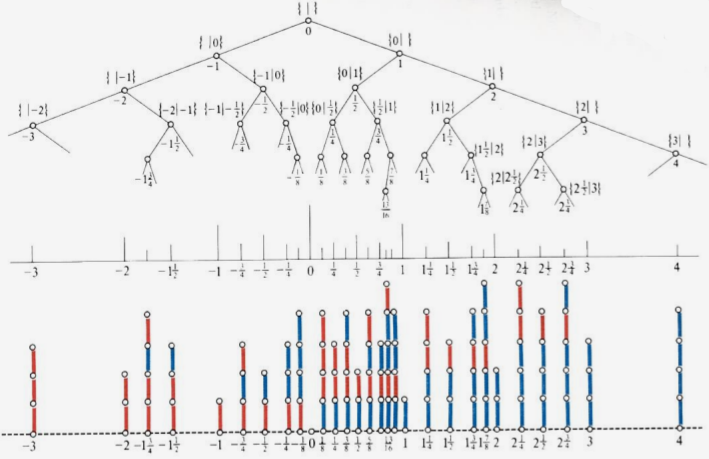
\includegraphics[width=\textwidth]{simple_numbers.png}
  \label{fig:simple_numbers}
\end{figure}

\begin{aufgabe}
 Versuche jetzt, den Wert für das Pferd in Aufgabe~\ref{auf_bewertungen} zu bestimmen, indem du alle möglichen Züge durchgehst, alle möglichen Stellungen bewertest (Wende dazu die Einfachheitsregel an!) und dir so langsam das Pferd zusammen baust. Es ist sehr effizient, an einer Kante in einer Skizze den Wert der Stellung zu schreiben, wenn man diese Kante entfernen würde.
\end{aufgabe}

\begin{aufgabe}
Wir betrachten folgende etwas seltsame Spielsituationen:
\begin{enumerate}
\item Ein Turm von unendlich vielen roten Kanten.
\item Ein Turm von unendlich vielen Kanten, bei denen die unterste (die, die mit dem Boden verbunden ist) rot und alle anderen blau sind.
\end{enumerate}
Wie lange dauern diese Spiele höchstens? Welcher Spieler besitzt Gewinnstrategien? Was passiert, wenn man in der ersten Situation endlich viele blaue Kanten dazustellt (jeweils nebeneinander)? Hast du eine Vermutung dafür, welche Bewertung diese Spiele haben?
\end{aufgabe}

% FALLS MAN NOCH WEITER GEHEN MOECHTE:
% \section*{Nimbers  und neutrales Hackenbusch}
% 
% Im Folgenden führen wir \emph{grüne} Kanten zusätzlich ein mit der folgenden Regel.
% \begin{itemize}
% \item Grüne Kanten dürfen von beiden Spielern entfernt werden. Sie sind also neutral.
% \end{itemize}
% Betrachten wir jetzt einmal die folgenden Situationen.
% 
% \begin{center}
% \begin{tikzpicture}
%     \draw[hline,black]  (0,0) -- (1,0);
%     \node[hnode] (g1) at (0.5,0) {};
%     \node[hnode] (g2) at (0.5,1) {};
%     \draw[hline,green] (g1) -- (g2);
%     
%     \draw[hline,black]  (1.5,0) -- (2.5,0);
%     \node[hnode] (a1) at (2,0) {};
%     \node[hnode] (a2) at (2,1) {};
%     \node[hnode] (a3) at (2,2) {};
%     \draw[hline,green] (a1) -- (a2) -- (a3);
%     
% %     \draw[hline,b\tikzstyle{hnode}=[draw,circle,inner sep=0,minimum size=3pt]
% \tikzstyle{hline}=[line width=1pt]lack]  (3,0) -- (5,0);
%     \node[hnode] (b6) at (3.5,0) {};
%     \node[hnode] (b7) at (3.5,1) {};
%     \node[hnode] (b8) at (4.5,0) {};
%     \node[hnode] (b9) at (4.5,1) {};
%     \draw[hline,green] (b6) -- (b7);
%     \draw[hline,blue] (b8) -- (b9);
% 
%     \draw[hline,black]  (5.5,0) -- (7.5,0);
%     \node[hnode] (d6) at (6,0) {};
%     \node[hnode] (d7) at (6,1) {};
%     \node[hnode] (d8) at (7,0) {};
%     \node[hnode] (d9) at (7,1) {};
%     \draw[hline,green] (d6) -- (d7);
%     \draw[hline,red] (d8) -- (d9);
% 
%     \draw[hline,black]  (8,0) -- (10,0);
%     \node[hnode] (e6) at (8.5,0) {};
%     \node[hnode] (e7) at (9.0,0) {};
%     \tikzstyle{hnode}=[draw,circle,inner sep=0,minimum size=3pt]
% \tikzstyle{hline}=[line width=1pt](e7) at (8.5,1) {};
%     \node[hnode] (e8) at (9.5,0) {};
%     \node[hnode] (e9) at (9.5,1) {};
%     \node[hnode] (e10) at (9.5,2) {};
%     \draw[hline,green] (e6) -- (e7);
%     \draw[hline,red] (e8) -- (e9);
%     \draw[hline,blue] (e9) -- (e10);
% 
%     \draw[hline,black]  (10.5,0) -- (12.5,0);
%     \node[hnode] (c1) at (11,0) {};
%     \node[hnode] (c2) at (12,0) {};
%     \node[hnode] (c3) at (11,1) {};
%     \node[hnode] (c4) at (12,1) {};
%     \node[hnode] (c5) at (12,3) {};
%     \node[hnode] (c6) at (12,2) {};
%     \draw[hline,green] (c1) -- (c3);
%     \draw[hline,red] (c2) -- (c4);
%     \draw[hline, blue] (c4) -- (c6) -- (c5);
% \end{tikzpicture}
% \end{center}
% 
% Wie man schnell merkt, gewinnt bei einem einzelnen grünen Stapel der anziehende Spieler, indem er einfach alle Kanten wegnimmt. Das heißt, dass der \emph{anziehende Spieler immer gewinnt}, dies ist also kein Nullsummenspiel! Schaut man sich jetzt die mittleren beiden Spiele an, sieht man $-1<X<1$, wenn $X$ eine einzelne grüne Kante bezeichnet. Von den letzten beiden Stellungen sieht man aber $-\frac{1}{2^n}<X<\frac{1}{2^n}$ für alle $n\in\NN$ indem man immer höhere Türme betrachtet und die Farben invertiert. Daraus folgt normalerweise $X=0$ (Warum?) aber wir wissen bereits $X\neq 0$.
% 
% Die Lösung dafür ist, dass wir eine neue ``Zahl'' einführen, und zwar
% \begin{equation*}
% \star:=
% \begin{tikzpicture}[baseline={(0,0.5)},scale=1]
%   \node[hnode] (g1) at (1,0) {};
%   \node[hnode] (g2) at (1,1) {};
%   \draw[hline,black]  (0,0) -- (2,0);
%   \draw[hline,green] (g1) -- (g2);
% \end{tikzpicture}
% =
% \left\{
% \begin{tikzpicture}[baseline={(0,0.05)},scale=1]
%   \draw[hline,black]  (0,0) -- (1,0);
% \end{tikzpicture}
% \middle|
% \begin{tikzpicture}[baseline={(0,0.05)},scale=1]
%   \draw[hline,black]  (0,0) -- (1,0);
% \end{tikzpicture}
% \right\} = \{0\mid 0\}.
% \end{equation*}
% Außerdem definieren wir rekursiv $\star0:=0=\{\;\mid\;\}$, $\star1:=\star$ und $\star n:=\{\star 0,\star 1, \star 2, \ldots,\star(n-1)\mid\star 0,\star 1,\star 2, \ldots, \star(n-1)\}$.
% \begin{aufgabe}
%   Welche Stellung entspricht den $\star n$?
% \end{aufgabe}
% Wegen der letzten Aufgabe ist $\star n$ die Berwertung der Stellung, die aus $n$ grünen aufeinander gestapelten Kanten besteht. In diesem Spiel kann jeder der Spieler eine beliebige Anzahl der Kanten wegnehmen und das Ziel ist, die letzte Kante selber zu entfernen. Das entspricht genau Nim auf einem Haufen, wenn man die maximale Zahl der entfernbaren Kanten ignoriert! Das heißt, dass (diese Version von) Nim ein Beispiel für Stellungen in \emph{neutralem Hackenbusch} ist.
% \begin{aufgabe}
%   Welchen Wert haben die folgenden Stellungen?
%   \begin{center}
%     \begin{tikzpicture}
%     \draw[hline,black]  (0,0) -- (2,0);
%     \node[hnode] (g1) at (0.5,0) {};
%     \node[hnode] (g2) at (0.5,1) {};
%     \node[hnode] (g3) at (1.5,0) {};
%     \node[hnode] (g4) at (1.5,1) {};
%     \draw[hline,green] (g1) -- (g2) (g3) -- (g4);
%     
%     \draw[hline,black]  (3,0) -- (5,0);
%     \node[hnode] (a1) at (3.5,0) {};
%     \node[hnode] (a2) at (3.5,1) {};
%     \node[hnode] (a3) at (3.5,2) {};
%     \node[hnode] (a4) at (4.5,0) {};
%     \node[hnode] (a5) at (4.5,1) {};
%     \node[hnode] (a6) at (4.5,2) {};
%     \draw[hline,green] (a1) -- (a2) -- (a3) (a4) -- (a5) -- (a6);
%     \end{tikzpicture}
%   \end{center}
% \end{aufgabe}
% Das zeigt
% \begin{equation*}
%   \star+\star=0.
% \end{equation*}
% Das besondere an dieser Gleichung ist, dass $\star\neq0$ gilt, aber dennoch $\star+\star=0$. Solche ``Zahlen'' oder eher algebraische Objekte tauchen in der Mathematik sehr häufig auf, nur sind sie nicht so gut vorstellbar, weshalb sie in der Schule ignoriert werden.
% 
% Die folgende Aufgabe zeigt ein paar Rechenregeln für $\star n$. Übrigens nennt man diese Werte auch \emph{Nimbers}, weil sie gewissermaßen Zahlen sind und sehr viel mit Nim zu tun haben.
% \begin{aufgabe}
%   Beweise die folgenden Rechenregeln:
%   \begin{enumerate}
%   \item $\star n+\star n=0$ für beliebige $n\in\NN$
%   \item $\star1+\star2=\star3$ \emph{Spiele die Stellung aus.}
%   \item $\star1+\star3=\star2$ \emph{Rechne mit a) und b).}
%   \item $\star1+\star4+\star5=0$ \emph{Spiele die Stellung und führe sie auf b) zurück.}
%   \item $\star2+\star4+\star6=0$ \emph{Spiele die Stellung und führe sie auf b) oder d) zurück.}
%   \item $\star3+\star5=\star6$ \emph{Rechne mit a), b), d) und e)}
%   \item $x+\star=\{x\mid x\}$ für alle (echten) Zahlen $x$
%   \end{enumerate}
% \end{aufgabe}
% 
% Zu guter Letzt noch ein kleiner Bonus: Nim ist ein neutrales Spiel. Es stellt sich heraus, dass Nim das universelle neutrale, endliche und normale Spiel mit vollständiger Information und ohne Zufall ist.
% \begin{thm}[Sprague--Grundy]
%   Jedes neutrale, endliche und normale Spiel mit vollständiger Information und ohne Zufall ist äquivalent zu Nim, wenn man zu Nim die folgende Regel hinzufügt:
%   \begin{itemize}
%   \item Anstatt in einem Zug Kanten zu entfernen, darf man einen Nim-Stapel um eine beliebige Anzahl von Kanten vergrößern, wobei die Kanten nur aus dem eigenen \emph{Vorrat} stammen dürfen. Der Vorrat besteht nur aus Kanten, die man selber in vorherigen Zügen entfernt hat.
%   \end{itemize}
% \end{thm}
% Dadurch kann man alle solchen Spiele (leider sind die meisten nicht sehr interessant) durch ihre Nimber-Werte beschreiben. Ein analoges Resultat für neutrales Hackenbusch existiert auch, wobei die Klasse der Spiele leider \emph{nicht} alle endlichen, normalen Spiele mit vollständiger Information und ohne Zufall ist.
\end{document}
